\documentclass{btswhitepaper}
\title{Smartcoins on the BitShares Blockchain}
\author{
 \IEEEauthorblockN{Fabian~Schuh}
 \IEEEauthorblockA{BitShares Europe, BitShares.eu\\
                   Erlangen, Germany\\
                   Email: \texttt{fabian@bitshares.eu}}
 \and
 \IEEEauthorblockN{Daniel~Larimer}
 \IEEEauthorblockA{Cryptonomex, Cryptonomex.com\\
                   Blacksburg (VA), USA\\
                   Email: \texttt{dan@cryptonomex.com}}%
 \thanks{This work was supported by Cryptonomex and honorable members of the
         bitsharestalk.org community.}
}


\begin{document}
\sloppy
\maketitle

\begin{abstract}%

 With the current growth of the crypto- ecosystem in general, and the
 growth of crypto- currencies like BTC (Bitcoin Blockchain) and ETH
 (Ethereum Blockchain) in particular, the general public as well as
 traditional (old economy) markets finally take notice of blockchain
 technology and its application(s) in the financial technology and other
 sectors. A well-known obstacle to greater adoption of crypto-currencies
 like BTC (Bitcoin) as a medium of payment is the high volatility of its
 exchange value, due to its limited supply. As a consequence, the unit
 price varies (sometimes significantly) over short periods of time. This
 makes BTC unpractical for merchants that need to pay their suppliers in
 cash, especially in bearish markets where this currency risk can ruin a
 business.

 A crypto-currency, with the properties and advantages of Bitcoin, that
 is capable of maintaining price parity with a globally adopted currency
 (e.g. U.S. Dollar), has high utility for convenient and cheap commerce.

 This document serves as a detailed and accurate description of so called
 \emph{smartcoins}, often also referred to as \emph{bitassets} or \emph{market
 pegged assets}. These refer to special kinds of tokens that are governed
 autonomously and transparently by the blockchain's internal smart contracts.
 Prominent examples are \textbf{bitUSD} and \textbf{bitCNY} which provide
 automation and incentives for market participants to maintain a high
 correlation with the value of U.S. Dollar or CNY.

\end{abstract}

\section       { Introduction                                     } \label{sec:mpa}
%%%%%%%%%%%%%%%%
% Smartcoins
%%%%%%%%%%%%%%%%
In today's world, crypto-currencies are unique because they are the only type
of digital currency that does not represent a corresponding counterparty
liability. Instead, they are \emph{fungible} and \emph{decentralized} tokens, whose
value is derived from the amount of practical utility (or potential future
utility) perceived by the network of users that support and trade in them.

Not surprisingly, most crypto-currencies suffer from high levels of price
volatility due to many complex factors, such as constantly shifting
public perception and highly speculative and unregulated markets.
Although professional traders tend to appreciate this volatility, so far
it has hindered the widespread adoption of cryptocurrency as a
\emph{practical payment solution}. A crypto-currency that has the
properties and advantages of Bitcoin, but is also capable of maintaining
price parity with a globally adopted currency (e.g. U.S. dollar), would
have incredible high utility for convenient and fast e-commerce.

The BitShares Blockchain offers a solution to this problem by introducing
\emph{smartcoins} - a framework for collateralized, counterparty risk-free loans
that enable token that highly correlate with the valuation of an
underlying asset, such as U.S. Dollar. Said framework is realized by a set of smart contracts
on the blockchain. 

Most prominent example of smartcoins on the BitShares Blockchain are 
\emph{bitUSD} and \emph{bitCNY}, which are smartcoins specific to one particular use
- namely to realize price-stable tokens. It is worth noting that that
price-stable tokens are merely one subset of possiblities within the
smartcoin framework. In literature, smartcoins are also often referred
to as \emph{bitassets} or \emph{market pegged asset}. 
\section       { Terminology                                      } In this paper we refer to \emph{smartcoins} as a means for customization of
tokens within a \emph{framework} of smart contracts and parameters as offered
by the BitShares Blockchain. In literature, smartcoins are also often referred
to as \emph{bitassets} or \emph{market pegged asset}.

As such, tokens like \emph{bitUSD}, \emph{bitCNY} and others are merely cases
specific to one particular use.
 

\section       { Smartcoin                                        } BitShares' market pegged assets (MPA), or \emph{Smartcoin} (as they is often also
called) are a new type of freely traded digital asset whose value is meant to
track the value of a conventional asset such as the U.S. dollar or 1 ounce
of gold. What makes market pegged assets unique is that they are free from
counter party risk.

A currency with the properties and advantages of Bitcoin that maintains price
parity with a globally adopted currency such as the US dollar has high utility
for convenient and censorship resistant commerce. A SmartCoin (synonym for
Market Pegged Asset) is a cryptocurrency that always has 100\% or more of
their value backed by the BitShares core currency, BTS, to which they can be
converted at any time at an exchange rate set by a trustworthy price
feed\footnote{Price feeds are published by delegates that have shareholder
approval.}. 
 
This paper will explain how market pegged assets including (for instance)
\emph{BitUSD} (intended to track the value of the US dollar) achieve price
parity while minimizing risk to holders.
 
\subsection    { Price Stability                                  } Ever since the bitcoin blockchain initiated the age of decentral public
ledgers, economists and engineers are trying to achieve a stable cryptocurrency
or a price pegged crypto token. The following two subsection want to discuss
the meaning of a ``stable'' currency and show how BitShares want's to fill the
gap.
 
\subsubsection { Definition of Price Stability                    } Before we discuss how BitShares achieves price \emph{stability} we first need to
define what properties make a currency \emph{stable}.

In the U.S., for instance, the Federal Reserve (FED) has a mandate of
\emph{stable prices} and it is almost universally accepted that this is a good
mandate. The same holds true for the Euro with its stability being
\emph{controlled} by the European Central Bank (ECB). Mostly every
country/nation or federation applies a similar concept.

However, it is also widely accepted among many crypto-currency fans that, in
the case of the US dollar, the FED has failed at their mandate because of
monetary inflation and increase in the money supply. Since monetary inflation
is a sustained increase in the general level of prices, it is equivalent to a
decline in purchasing power of money. Hence, a dollar buys less and less over
time. As a result, we see the dollar losing 99\% of its \emph{purchasing power}
since the FED was founded in 1913~(see \cref{fig:monetarybase}). 

\begin{figure}[!htp]
 \centering
 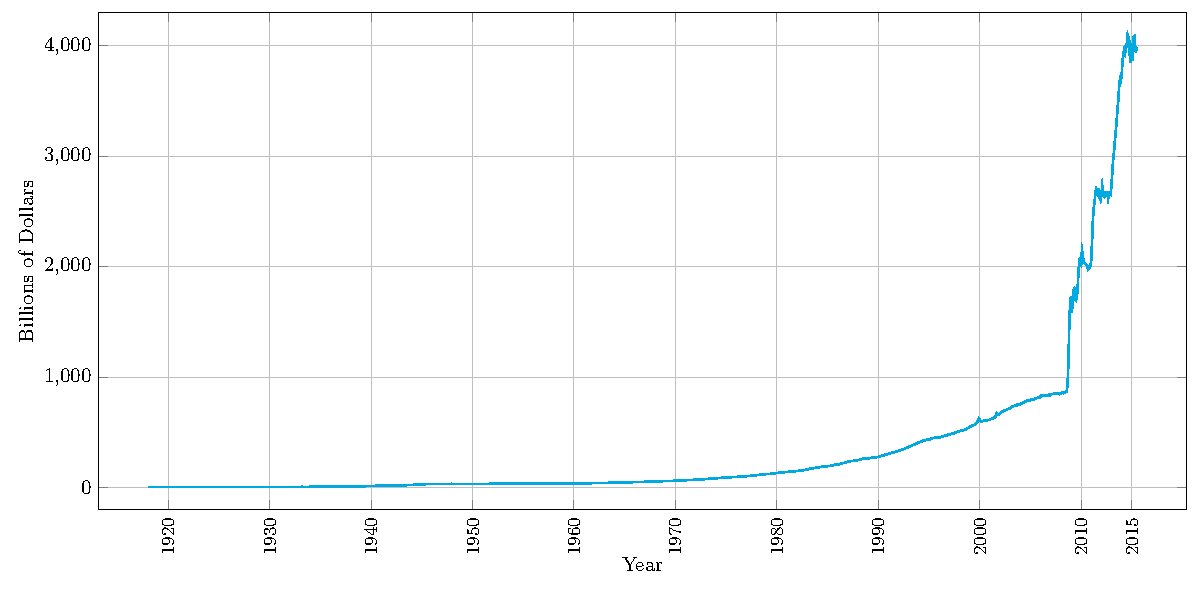
\includegraphics[width=\linewidth]{figures/monetary-base}
 \caption{St. Louis Adjusted Monetary Base~\cite{ambsl}}
 \label{fig:monetarybase}
\end{figure}

The goal of this paper is not to propose a replacement of central banks but to
clarify the terminology in particular with regards to ``stable''
cryptocurrencies. Unfortunately, some people in the cryptocurrency space are
attempting to provide an alternative currency that can achieve the same
mandate. However, since price stability at its heart is the same as \emph{price
fixing}, this is a well known economic fallacy that crypto-currencies should
avoid.

% The goal of the FED price stability mandate is to mask the systematic theft of
% all increases in the production efficiency of the economy. 

Imagine a central bank managed to keep prices stable through their monetary
policy with 0\% price inflation over 20 years. Now lets assume that during this
same 20 years the advances in robotics and automation resulted in a 3x increase
in efficiency and thus there are now 3x as much food, cars, phones, houses,
etc. For the sake of this example we will assume the population is the same and
everyone has the same amount of money in the bank. You would normally expect
that everything would be 1/3 the price and that everyone would be able to
afford 3x their prior life style. But because of the central bank's
intervention they have managed to also increase the money supply by 3x.
% and distribute it in secret. The end result is that some people get a 1000x
% increase in life style while everyone else stands still.

% FIXME: not very neutral!
% We can conclude from this example that the mandate for price stability is
% mostly a goal meant to mislead the general public and mask theft from the lower
% and middle classes on a massive scale even at 0\% price inflation. For this
% reason, we do not want to bring this same mandate to crypto currencies but
% instead aim to free us from monetary enslavement.

We notice that the goals should not be \emph{price stability} nor should we
target a \emph{stable value} or \emph{purchasing power} (at least not yet). 
%
What we want to achieve instead is 
\begin{itemize}
 \item a \emph{predictable} price with \emph{reduced volatility}
 \item a somewhat reliable ability to \emph{predict the future value} of a token, and
 \item a unit of account that doesn't have any meaningful capital gains or
       losses for tax purposes.
\end{itemize}

Hence, price ``stability'' really means price \emph{predictability} within some
tolerance level. In the case of the U.S. dollar, a willingness to accept a 5\%
loss (in purchasing power) per year via deflation, demonstrates that
predictability is more important than stability~\cite{bm:stable:impossible}.
 
\subsubsection { BitAssets 1.0: Historical Lessons                } \label{sec:bitassets1}

The first proposal of the BitAsset system has evolved over 9 months since it
first launched as we learned how market participants reacted to various rules.
We notices that, liquidity is critical to confidence in the value of the token
and that a system with unbalanced rules will tend to bias the price in one
direction or the other.

Early on, BitUSD was driven down to \$0.85 as demand for shorting outstripped
demand for BitUSD and shorts were not forced to cover. Then, after implementing
a \emph{30 day forced covering rules}, the price stabilized around \$0.98 to
\$1.00. Later, as the cryptocurrency bear market progressed, we had BitUSD
trading at \$1.05 or more because everyone is scared to use leverage and those
that have open positions looked to cover their position while those who held
BitUSD were not looking to sell. Over the course of these past 9 months, we
have seen 3 different markets and had an opportunity to better understand the
behavior of market participants and improve the protocol accordingly.

We have seen that the idea of a market pegged crypto token can in general work,
but obviously, we were not satisfied as to \emph{how well} BitAssets 1.0
worked. For that reason, the improved BitAssets 2.0 protocol was proposed which
will be described in the following.
 
\subsubsection { BitAssets 2.0: Evolving a Stable Crypto Currency } For BitUSD to be accepted as being equal to \$1.00 for the purposes of setting
prices, it only needs to maintain a \emph{floor} of \$1.00. If it can maintain
a floor of \$1.00, then merchants can accept it and know their margins are safe
and that they are \emph{not exposed to currency risk}. In order to enable a
guaranteed floor, all BitUSD can be \emph{force liquidated} at a trustworthy
price feed\footnote{Price feeds are published by \emph{witnesses} that have
shareholder approval. See~\cref{sec:feeds}.}. Since this rule is present,
those who create the BitUSD must sell it at a price that properly accounts for
this risk of \emph{forced settlement}. This means that at almost all times, new
BitUSD will only enter circulation when there is a buyer willing to pay a
premium for a guaranteed floor.

As we will see, since USD holders can initiate settlement, there is no need for
artificial forced covering every 30 days. This relieves shorts of risk, helps
increase short demand, and keeps the price of BitUSD near the floor.
 
\subsection    { Autonomy and Transparency                        } 
\subsection    { Parameterization                                 } 
\subsection    { Ownership and Responsibilities                   }

\section       { Mechanics                                        } \label{sec:mpa:create}

A BitShares MPA can be viewed as a contract between an asset buyer seeking
price \emph{stability} and a short seller seeking greater \emph{exposure} to
BTS price movement. The open source BitShares software protocol implements a
decentralized marketplace for MPA where all transactions are recorded on the
shared block chain ledger and the software enforces the market rules. This
block chain based marketplace is referred to as the \emph{decentralized
exchange} or \emph{internal market} (c.f., \cref{sec:dex}) to distinguish from
\emph{external markets} such as websites that facilitate the exchange of
government issued currencies with cryptocurrency.

SmartCoins are tokens of a particular MPA (e.g. bitUSD). They use the concept
of a contract for difference, and make the long side fungible. For the purpose
of this discussion, we will assume that the long side of the contract is BitUSD
and that the backing \emph{collateral} is BTS (the BitShares core asset).

In practice, bitUSD are created on the BitShares blockchain when a BTS holder
asks the network for them by handing over \emph{collateral} to the network,
essentially locking them in a contract for difference (c.f., \emph{1)} in
\cref{fig:btsdex}).

\begin{figure}[!htp]
 \begin{center}
  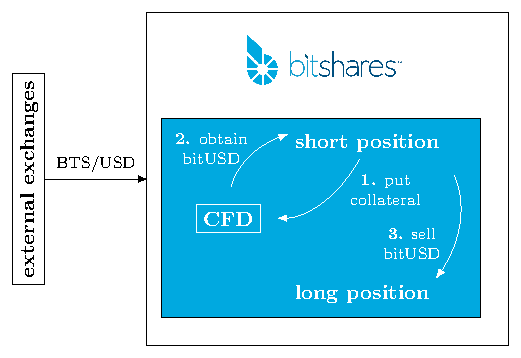
\includegraphics[width=.8\linewidth]{figures/external-pricefeed}
 \end{center}
 \caption{Illustration of external price discovery and a ``short sell'' to seek
          greater exposure for BTS price movements.}
 \label{fig:btsdex}
\end{figure}

The collateral is only returned to the short seller when the corresponding
amount of the asset agreed in the contract is handed over to the BitShares
network again. The protocol will then effectively destroy these tokens and
fulfill the contract. This is referred to as \emph{covering a
short}. At the moment of creation, the position of the \emph{shorter} has not
changed at all because he can directly cover his own short position using the
bitUSD to gain back his BTS used as collateral.

If the short seller has sold the SmartCoins he has created, then he would be
required to purchase them back from the market before closing his short
position. Meanwhile, if the value of the collateral relative to the current price
of the market pegged asset falls below a certain margin of safety, the assets
can be automatically (i.e. initiated by the protocol itself) repurchased from
the market before the collateral becomes insufficient.

These rules create systemic demand for market pegged assets while allowing them
to remain fungible. To protect your contract against \emph{margin calls}
(automated, network initiated force settlement of your contract at the price
feed), you should at least maintain the so called \emph{maintenance collateral
level} at all times. Hence, the collateral only needs to be high enough to
cover any slippage as a result of a short squeeze.

In summary, the following set of market rules apply to all market pegged assets
(for the sake of simplicity, we here focus on the MPA bitUSD):
\begin{itemize}
 \item Anyone with BitUSD can settle their position within an
       interval\footnote{defined by the shareholder approval} at the settlement
       price (identical to the feed price).
 \item In this case, the \emph{least} collateralized short positions would be
       margin called and their collateral would be used to settle the position.
 \item The price feed is the median of many sources that are updated at least
       once per hour.
 \item Short positions never expire, except by hitting the maintenance
       collateral limit, or being force-settled as the least collateralized at the
       time of forced settlement (see point 2).
 \item In the event that the least-collateralized short position lacks enough
       collateral to cover at the price feed, then all BitUSD positions are
       automatically force settled at the price of the least collateralized
       short (black swan event, see~\cref{sec:blackswan}).
\end{itemize}

These simple rules enable a price floor of \$1.00 for 1.00 BitUSD. A simple
metric for testing the validity of our claim is to demonstrate that, if you can
find someone willing to sell 1.00 BitUSD for \$1.00, that it would be the
cheapest option for buying BTS. This means that 100\% of the buying demand for
BTS would be available to give liquidity to BitUSD holders as a priority over
BTS holders.
 
\subsection    { Face Value                                       } 
\subsection    { Price Feeds                                      } \label{sec:feeds}

The blockchain needs to be aware of the external price of BTS in order for
settlements to convert SmartCoins into the core asset (BTS) at a fair price.

In BitShares, this is achieved by means of a set of $N$ trusted
\emph{witnesses}. These witnesses have to be elected by the corresponding
BitShares shareholders (e.g. holders of BTS) and can be constantly reviewed as
all prices are put on the blockchain in a public manner by means of
transactions of a certain type. Hence, misbehaving witnesses can be identified,
``fired'' and lose their reputation of shareholders.

Additionally, to prevent manipulation of the price feed, $N$ witnesses have to
be elected that can all produce their prices independently. Having a set of $N$
prices $p_i,\;1<i<N$ for an arbitrary MPA on the blockchain, the protocol
obtains a single price $\tilde{p}$ by the use of the \emph{median} according
to:
\begin{align}
 x &= \operatorname{sort}(p[i])\\
 \tilde p &=\begin{cases}
   x[\frac{N+1}{2}]                                               & N \text{ odd}\\
   \frac {1}{2}\left(x[{\frac{N}{2}}] + x[\frac{N}{2} + 1]\right) & N \text{ even.}
 \end{cases}
\end{align}
Hence, the price is resistant against misbehaving witnesses in that only a
majority of price publishers can manipulate the outcome of the median. In
practice, any unintentional feed \emph{error} is thus balanced around the true
price. % FIXME later, show some statistics from bts-0.9

Obviously, the shareholders are required to constantly monitor the published
prices of their witnesses and should make a public note about any
discrepancies. This is similar to traditional \emph{quality management} for the
\emph{Smart Coin} products (e.g. bitUSD) and BitShares system can offer a paid
position to perform this service.
 
\subsubsection { Price Manipulation                               } There is always concern of price manipulation. Someone with a large amount of
money on both sides of a trade can use their funds to manipulate the markets
and thus the price feed. If the amount of money they lose manipulating the
markets is less than the amount of money they can gain by manipulating the
price feed, then it will be profitable to manipulate the market at the expense
of either the BitUSD longs or the shorts. A low-collateralized short that sees
a large force-settlement order requested can attempt to manipulate the markets
and thus the feed against the BitUSD holder.

The risk of price manipulation is priced into the premium on BitUSD charged by
the shorts, and thus should already be priced into the market. If price
manipulation became a serious problem that caused very high premiums, then it
could be addressed by the price feed producers, who can adopt a moving average
over wider time windows to increase the difficulty of short-term manipulation.
A variety of algorithms could be used to estimate a ``fair price'' that keeps
BitUSD valued at least \$1.00.

In practice, a feed producer can observe the BitUSD-to-USD market as an
indicator on which way to adjust the feed. Generally speaking, the strategy
that the feed producers adopt for controlling the feed should be public
knowledge, because the shorts will ultimately rely on it. For the feed
producers to change strategies in unpredictable ways could cause losses to both
longs and shorts.
 
\subsection    { Collateralization                                } 
\subsection    { Settlement                                       } 
\subsection    { Margin Calls                                     } 
\subsubsection { Calling for insufficient collateral }
\subsubsection { Margin Call Orders }
\subsubsection { Order of Filling }
\subsection    { Global Settlement                                } All guarantees of SmartCoins are subject to the caveat that a SmartCoin can
never be worth more than the collateral backing the least-collateralized short
position. In normal market conditions, the value of the collateral is always
more than sufficient, but, from time to time, markets can rapidly revalue the
collateral. If this revaluation happens faster than the short positions can be
forced to cover, then all SmartCoins are liquidated at the exchange rate of the
least collateralized short position. This is similar to an insolvent bank
converting its deposits to equity.
 

\subsection    { Risks                                            } The current implementation of market pegged assets in the BitShares system is
designed to minimize risk of loss to market pegged asset holders. Short
positions are opened with collateral worth three times the market value of the
asset. The initial collateral is comprised of the BTS paid by the buyer for the
asset and twice this amount of BTS contributed by the short seller. The
collateral requirements and margin triggers were chosen conservatively to
protect the holders of market pegged assets from volatility of the underlying
collateral. Forcing short positions to cover every 30 days provides additional
assurance of short term liquidity. Control over the price feed is distributed
among over 50 separately elected delegates who compile information from
multiple exchange sources. Despite such precautions, it is important to
carefully explore risks of using the system. Risks can be broadly categorized
as value risk, counterparty risk, or systemic risk.
 
\subsubsection { Collateral Risk                                  } Market pegged assets maintain their price parity due to being backed by
collateral that has an established real world value. When the value of the
collateral falls, the system is designed to react by driving the internal asset
exchange to match the new real world exchange rate and trigger \emph{force
settlements} (also known as margin calls) if necessary.

% First half of the paragraph contains dublicated information from
% fp-mpa-blackswan.tex
However, there exists a possibility that the underlying collateral (BTS) drops
in value so quickly the market pegged assets become under-collateralized. Often
termed a \emph{black swan event} (c.f., \cref{sec:blackswan}), a sudden crash
of BTS value could prevent the system from adjusting in time. In this event,
the full amount of collateral is no longer sufficient to purchase the market
pegged asset back at the new real exchange rate. In such an event, assets may
settle at the price fees and are converted back into the underlying collateral
(BTS). This may expose customers at the volatility risk of BTS. Under normal
conditions, short term market movements, spreads, and fees charged by exchanges
may also affect the potential cost of conversion into and out of market pegged
assets.
 
\subsubsection { Counterparty Risk                                } Unlike many attempts to create a digital asset that tracks the dollar, market
pegged asset are not an ``\emph{I owe you}'' issued by any entity. For this
reason, it does not rely on a specific counterparty to honor its value (unless
you choose to view the software protocol itself as an independent
``counterparty'' entity). 

Although manipulation risk occurs in any market, it is minimized by the open
source and auditable nature of the BitShares system and carefully considered
market rules. MPAs stored on a \emph{centralized} exchange become IOUs and are
subject to counter party risk~\cite{mtgox}. This risk is not a property of the
MPA themselves. We recommend that users never deposit their tokens on an
exchange and instead only use gateways that issue their IOUs onto the BitShares
network. This way you can trade your BitUSD against gateway IOUs without
exposing your BitUSD to counter party risk while in the order book (more
details in \cref{sec:gateway}).
 
\subsubsection { Systemic Risk                                    } Systemic risk is a catch-all for other risks required to utilize the system.
The primary risk is individuals are responsible for protecting the
cryptographic private keys that sign transactions proving ownership of assets.
These keys must be protected from theft or loss. This risk can be greatly
reduced and virtually eliminated by following best practices.

Systemic risk also includes the possibility of an overlooked fatal flaw in the
open source software or the possibility of large scale failure of global
network infrastructure and should reduce over time.
 
\subsection    { Privatized SmartCoins                            } Alternatively to regular MPA like the bitUSD, BitShares also offers
entrepreneurs an opportunity to create their own SmartCoins with custom
parameters and a distinct set of price feed producers.

User-issued SmartCoin managers can experiment with different parameters such as
collateral requirements, price feeds, force settlement delays and forced
settlement fees (see \cref{sec:uia:priv}). They also earn the trading fees from
transactions the issued asset is involved in, and therefore have a financial
incentive to market and promote it on the network. The entrepreneur who can
discover and market the best set of parameters can earn a significant profit.
The set of parameters that can be tweaked by entrepreneurs is broad enough that
SmartCoins can be used to implement a fully functional prediction market with a
guaranteed global settlement at a fair price, and no forced settlement before
the resolution date.

Some entrepreneurs may want to experiment with SmartCoins that always trade at
exactly \$1.00 rather than strictly more than \$1.00. They can do this by
manipulating the forced settlement fee continuously such that the average
trading price stays at about \$1.00. By default, BitShares prefers fees set by
the market, and thus opts to let the price float above \$1.00, rather than
fixing the price by directly manipulating the forced settlement fee.
 


\section        { Conclusion                                       } \input { content/fp-smartcoins-conc     }
\bibliographystyle{IEEEtran}
\bibliography{literature}
\end{document}
